\iffalse 

TODO : 
参考文献修正、フッターに書く?
リストのマークを変える、サイズ大きく
本文文字太くする?
画像があるといい

\fi

\RequirePackage{plautopatch} 
\documentclass[17pt,aspectratio=169]{beamer} 
\usepackage{amsmath}
\usepackage{amssymb}
\usepackage{graphicx}
\usepackage{luatexja}
\usepackage{luatexja-fontspec} 
\usepackage{fontspec}
\usepackage{color} 
\usepackage{tcolorbox}
\usepackage{ascmac}
\usepackage{bm} 
\usepackage{appendixnumberbeamer}
\usepackage{comment}

\usepackage{enumitem}
\setlist[itemize,1]{label=\textbullet, itemsep=17pt}  % 記号をもうちょっと大きくしたい
\setlist[itemize,2]{label=\textasteriskcentered, itemsep=3pt} 
\setlist[itemize,3]{label=\textendash, itemsep=3pt} 

\usetheme{metropolis}  % Metropolisテーマを使用
\setmainjfont{Yu Gothic Bold}  
\setsansjfont{Yu Gothic Bold}  

%Beamerフォント設定 
\usefonttheme{professionalfonts} % Be professional!
\usepackage[T1]{fontenc}
\usepackage{mlmodern}  % 太いComputer Modern
% MLmodernのバグを修正: cf. https://tex.stackexchange.com/questions/646333/size-of-integral-symbol-in-section-header-with-mlmodern
\DeclareFontFamily{OMX}{mlmex}{}
\DeclareFontShape{OMX}{mlmex}{m}{n}{%
   <->mlmex10%
   }{} 
\renewcommand{\familydefault}{\sfdefault}  % 英文をサンセリフ体に
\renewcommand{\kanjifamilydefault}{\gtdefault}  % 日本語をゴシック体に
\usefonttheme{structurebold} % タイトル部を太字
\setbeamerfont{alerted text}{series=\bfseries} % Alertを太字
\setbeamerfont{section in toc}{series=\mdseries} % 目次は太字にしない
\setbeamerfont{frametitle}{size=\large} % フレームタイトル文字サイズ
\setbeamerfont{title}{size=\LARGE} % タイトル文字サイズ
\setbeamerfont{date}{size=\normalsize}  % 日付文字サイズ
\setbeamerfont{author}{size=\normalsize}  % 日付文字サイズ
\setbeamerfont{normal text}{series=\mdseries} % 本文を太字に 

%ページ番号の設定
\setbeamertemplate{footline}{
    \hfill {\textcolor{gray!90}{\insertframenumber/\inserttotalframenumber}\hspace{0.1cm}}
    \vspace{0.1cm} 
}

%短縮形
\newcommand{\Pbb}{\mathbb{P}}
\newcommand{\Gcal}{\mathcal{G}}
\newcommand{\Fcal}{\mathcal{F}}

%タイトル
\title{¬ACの相対的無矛盾性証明のIsabelle/ZFによる形式化}
\author{東北大学 大学院情報科学研究科 住井・松田研究室 M2\\ 舟根大喜}
\date{November 22, 2024}

\begin{document}
\maketitle

\begin{frame}{概要}
    \begin{itembox}[l]{やったこと}
        \begin{center}
        $\neg$ACのZF上の相対的無矛盾性証明を\\
        Isabelle/ZFで形式化
        \end{center}
    \end{itembox}
    {\small
    \begin{itemize}[itemsep=8pt]
        \item 定理証明支援系を用いて\\
        数学の形式化をする試みが行われている
        \item 公理的集合論の中でも強制法(後述)を用いた議論の\\形式化はあまりないので貢献したい
    \end{itemize}}
\end{frame}

\begin{frame}{用語}\,
    \vspace{-20pt}
    {\small 
        \begin{itemize}[itemsep=8pt]
            \item \textcolor{red}{公理的集合論} \\
            \ldots 何が集合かを公理で厳密に定めて展開する集合論
            \item \textcolor{red}{ZF}
            \ldots Zermelo-Fraenkel公理系。最も一般的な公理系の一つ
            \item \textcolor{red}{AC} \ldots 選択公理 (Axiom of Choice)\\
            任意の非空集合の族からそれぞれ1つの元を選ぶ関数が\\存在するという公理
        \end{itemize}
    }
\end{frame}

\begin{frame}{用語}\,
    \vspace{-20pt}
    {\small 
        \begin{itemize}[itemsep=8pt]
            \item 命題$\varphi$が公理系$T$上で\textcolor{red}{相対的無矛盾} \\
            \ldots $T$が無矛盾ならば公理系$T+\varphi$も無矛盾であること
            \item $\varphi$が$T$から\textcolor{red}{独立} \\
            \ldots $T$から$\varphi$も$\neg\varphi$も証明できないこと \\
            \,\,\,\,\,\,\,($T$が無矛盾なら)$\varphi$と$\neg\varphi$のT上の相対的無矛盾性と同値
        \end{itemize}

        相対的無矛盾性を調べることで\\公理系の(無矛盾性の)強さを比較できる
    }
\end{frame}

\begin{frame}{用語}\,
    \vspace{-20pt}
    {\small 
    \begin{itemize}[itemsep=8pt]
        \item \textcolor{red}{強制法} \ldots \\
        集合論のモデルを拡張して新しいモデルを作る技法。\\
        $M$を強制法で拡張したモデルを$M$の\textcolor{red}{generic extension}と\\
        呼び、$M[G]$とかく(ここで$G$はgeneric filter) \\
        \,\\
        generic extension上で何が成り立つかは \\
        \textcolor{red}{強制関係}と呼ばれる関係\textcolor{red}{$\Vdash$}によって調べることができる
    \end{itemize}
}
\end{frame}
\section{Isabelle/ZFについて}

\begin{frame}{定理証明支援系}
    \begin{columns}
        \begin{column}{0.65\textwidth}
            \begin{itemize}[itemsep=7pt]
                \item 数学的証明の形式化や、\\ソフトウェアの正しさの証明\\などに用いられるシステム
                \item プログラムを書くように\\定義・証明を記述する
                \item Isabelle,Lean,Coq, \ldots
            \end{itemize}

        \end{column}
        \begin{column}{0.35\textwidth}
            \begin{figure}
                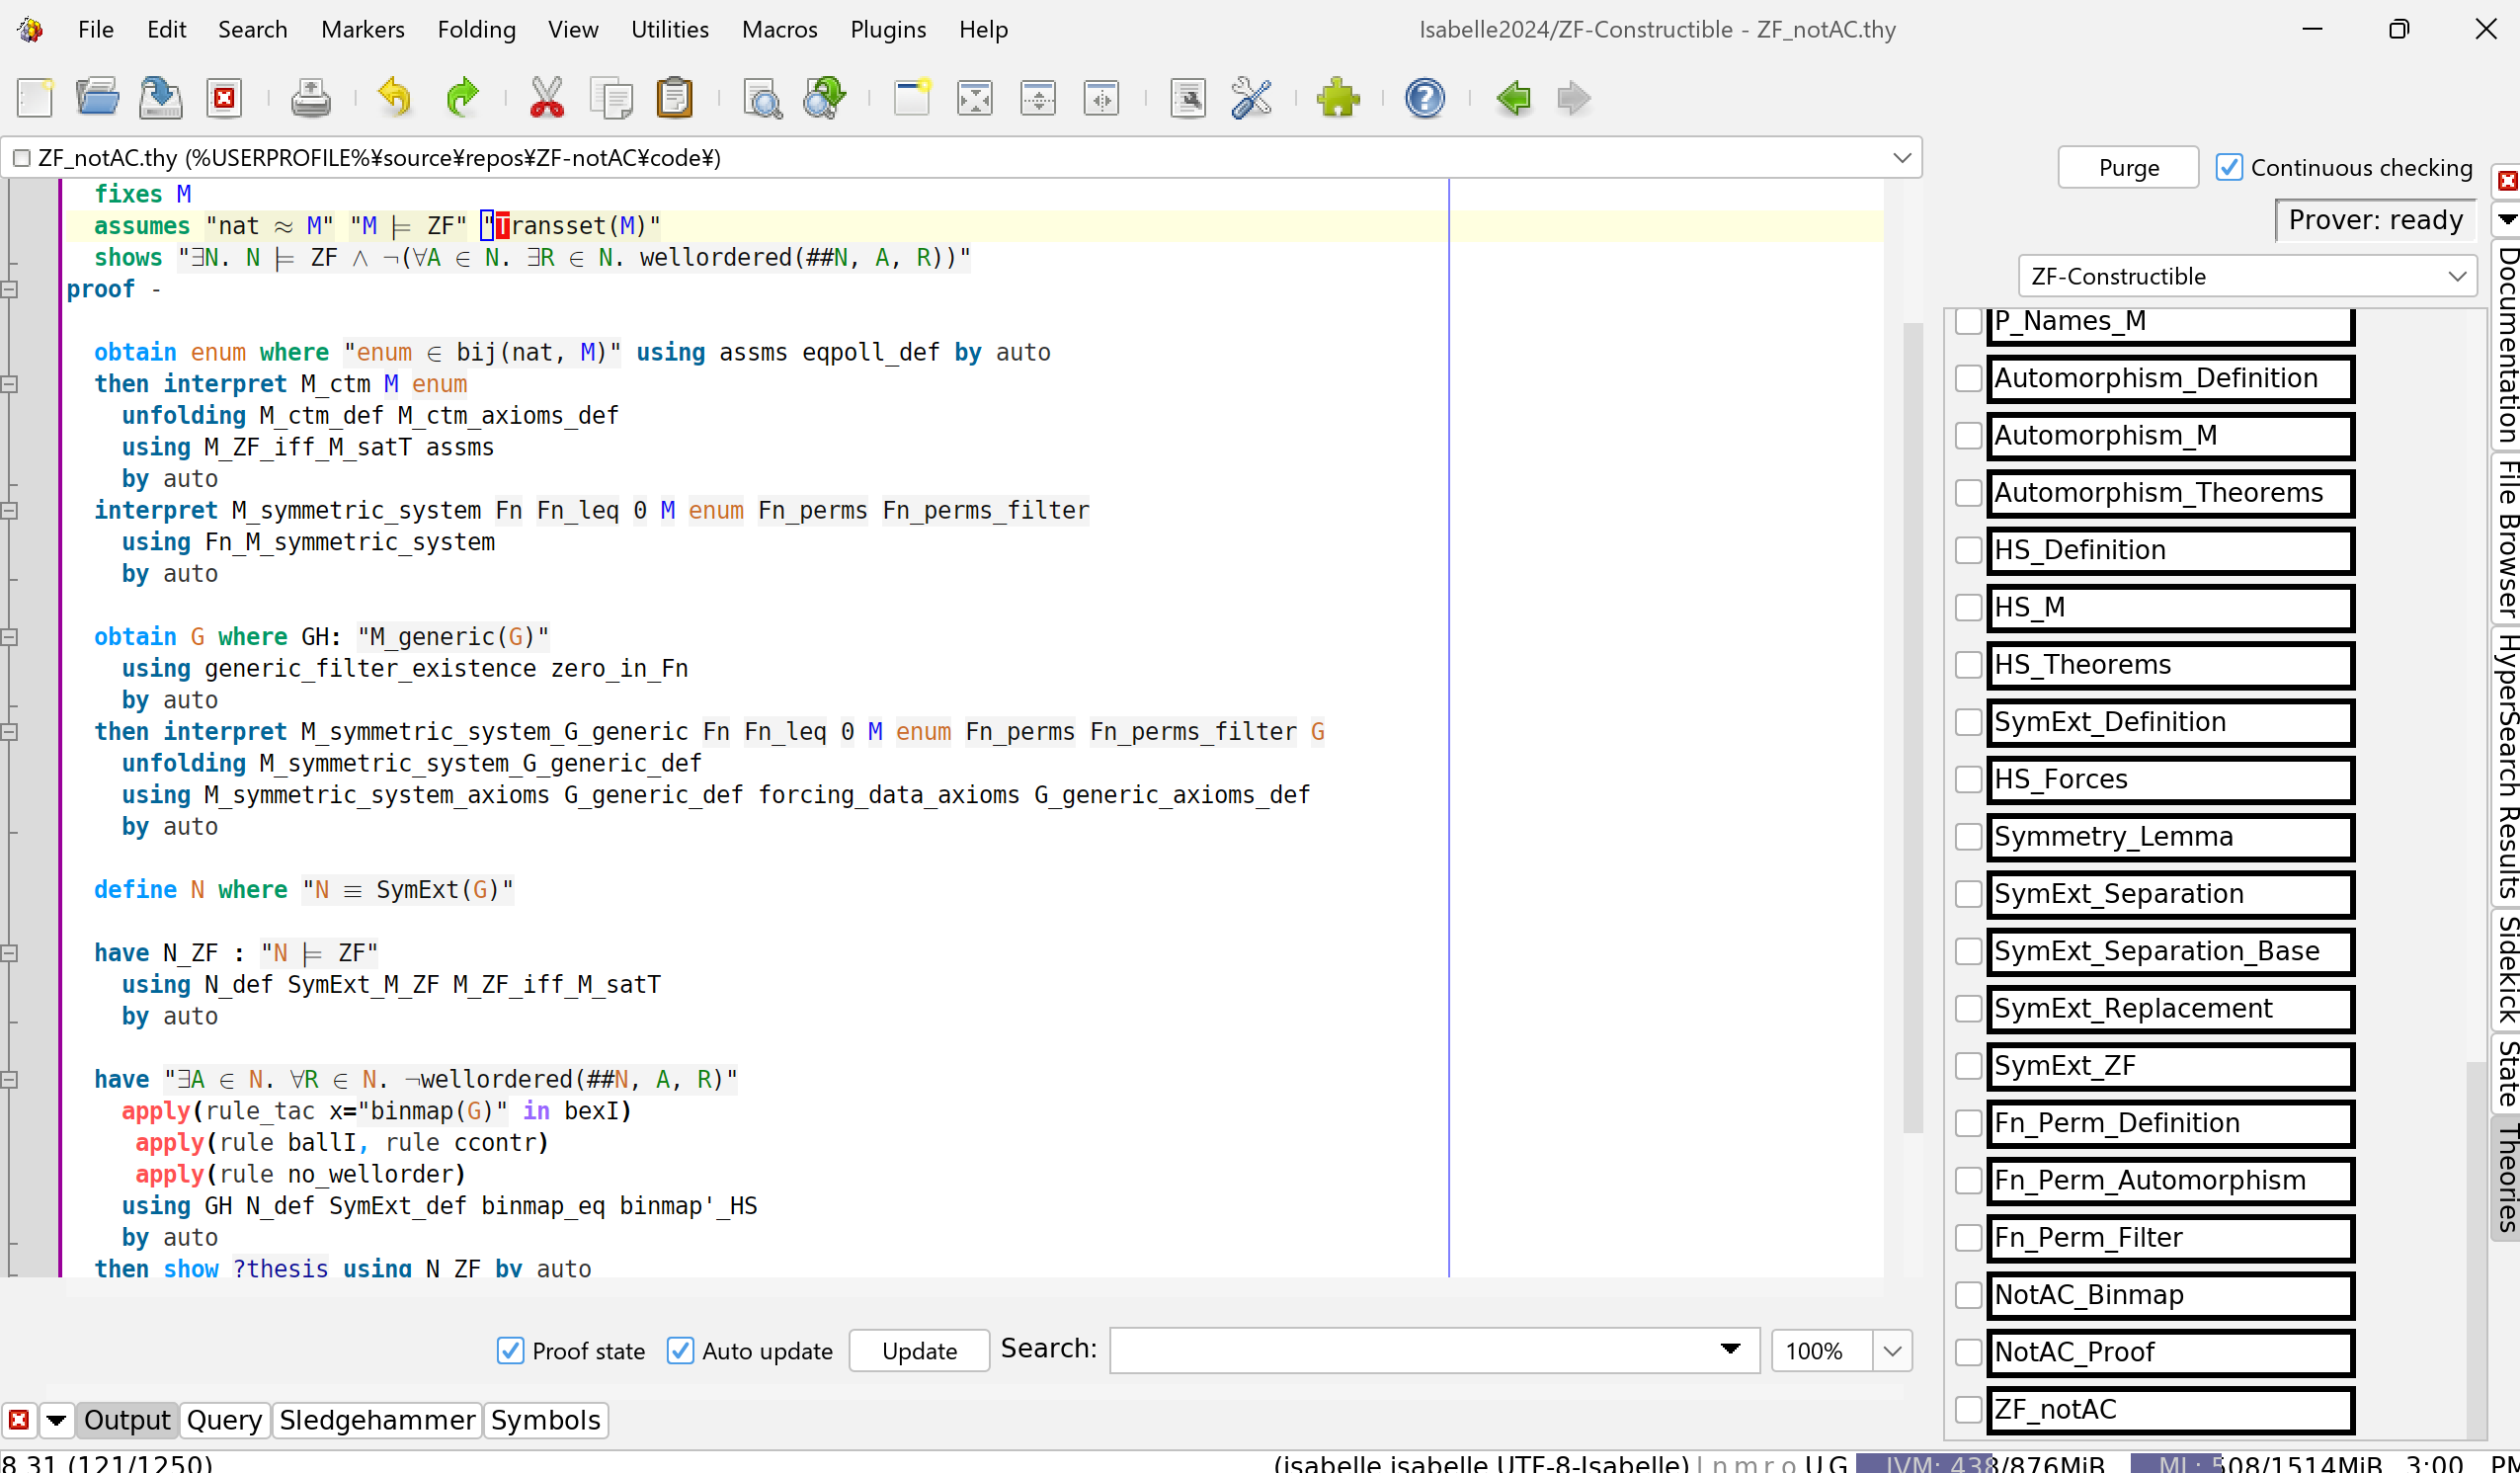
\includegraphics[width=1.0\linewidth]{./images/isabelle_editor.png}
            \end{figure}
            \vspace{-10pt}
            \begin{columns}
                \begin{column}{0.4\textwidth}
                    
\includegraphics[width=1\linewidth]{./images/lean.png}
                \end{column}
            \end{columns}
            \vspace{-10pt}
            \begin{columns}
                \begin{column}{0.4\textwidth}
                    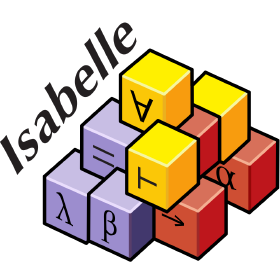
\includegraphics[width=1\linewidth]{./images/isabelle_logo.png}
                \end{column}
                \begin{column}{0.4\textwidth}
                    
\includegraphics[width=1\linewidth]{./images/coq.png}
                \end{column}
            \end{columns}
        \end{column}
    \end{columns}

    %----------------------------------------------
    % coqの画像 https://ja.wikipedia.org/wiki/Coq#/media/%E3%83%95%E3%82%A1%E3%82%A4%E3%83%AB:CoqProofOfDecidablityOfEqualityOnNaturalNumbers.png
    %----------------------------------------------

\end{frame}

%----------------------------------------------
%    マイクロカーネル
%    https://read.seas.harvard.edu/~kohler/class/cs260r-17/klein10sel4.pdf
%----------------------------------------------

\begin{frame}{Isabelle {\small [Paulson 86]}}
    \vspace{-5pt}
    \begin{itemize}[itemsep=3pt]
        \item 実績の例 : \\
            seL4カーネルの形式検証 {\small \,[Klein et al. 14]}
            \vspace{-3pt}
            \begin{itemize}[itemsep=2pt]
                \item 130万行の証明
            \end{itemize}
        \item Archive of Formal Proofs
    \end{itemize}
    
    \begin{columns}
        \begin{column}{0.25\textwidth}
            \begin{figure}
                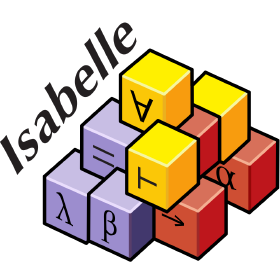
\includegraphics[width=0.7\linewidth]{./images/isabelle_logo.png}
            \end{figure}
        \end{column}
        \begin{column}{0.25\textwidth}
            \vspace{-7pt}
            \begin{figure}
                
\includegraphics[width=0.9\linewidth]{./images/sel4-logo.png}
            \end{figure}
        \end{column}
        \begin{column}{0.35\textwidth}
            \vspace{-20pt} 
            \begin{figure}
                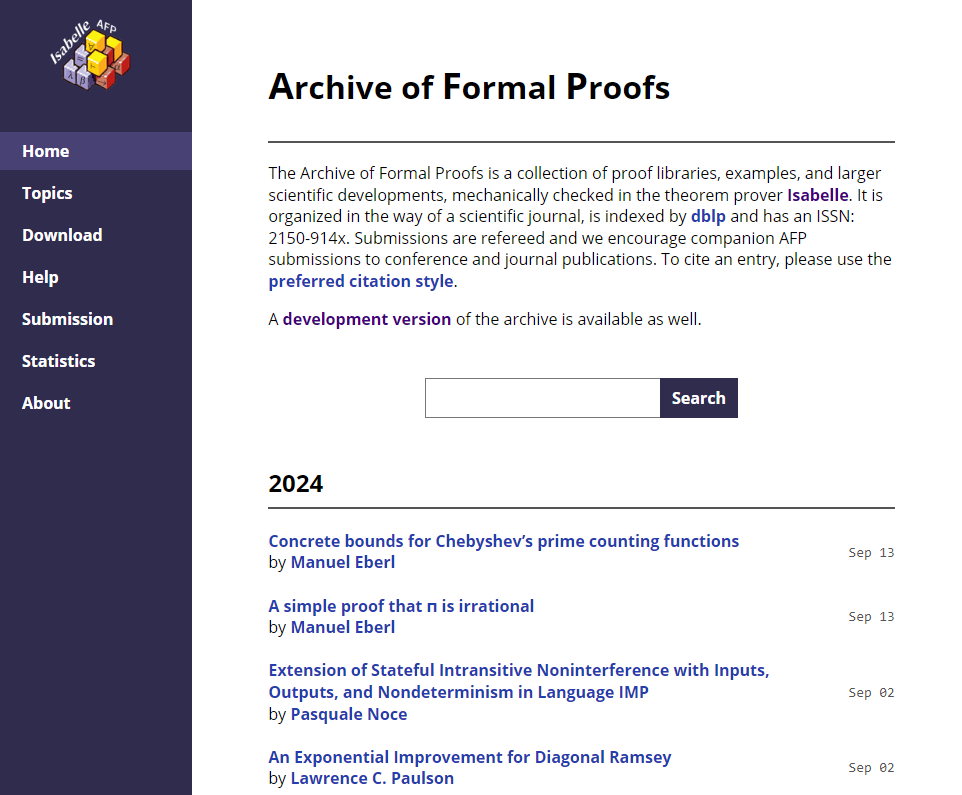
\includegraphics[width=0.8\linewidth]{./images/isabelle_archive.png}
            \end{figure}
        \end{column}
    \end{columns}
\end{frame}

\begin{frame}{Isabelle}
    \begin{itemize}
        \item 論理体系「Pure」上で定理証明を行う
        \item 「Pure」上に他の論理体系が構築されている
              {\small \begin{itemize}
                  \item Higher-Order Logic
                  \item First-Order Logic \\
                  \item \dots
              \end{itemize} }
              \vspace{-10pt}
        \item \textcolor{red}{Isabelle/ZF} $\cdots$ \\ 
        一階述語論理とZF(C)公理系のフレームワーク
    \end{itemize}
\end{frame}

% 簡単な定理証明の例を紹介するといいかも
% apply-script, structured proofの説明

% ZFの公理を記述しているコードを紹介するといいかも
% https://isabelle.in.tum.de/dist/library/FOL/ZF/ZF_Base.html ZFの公理のコード

\begin{frame}{Isabelle/ZFにおける先行研究}
 
    \begin{itemize}[itemsep=8pt]
        \vspace{10pt}
        \item CHのZFC上の独立性証明{\small [Gunther et al. 20,22]}
            \vspace{3pt}
              {\small \begin{itemize}
                \item 強制法の形式化 (13K行)
                \item CHの独立性証明 (16K行) ※Leanにも形式化がある
              \end{itemize} }

        \item ACのZF上の相対的無矛盾性証明{\small [Paulson 02]}
              {\small \begin{itemize}
                      \item 構成可能宇宙を形式化 (12K行)
                  \end{itemize} }
              % https://arxiv.org/pdf/2001.09715 強制法の形式化
              % https://cs.famaf.unc.edu.ar/~pedro/forcing/Independence_CH/document.pdf CHの独立性証明
    \end{itemize}
    \begin{itemize}
        \item [\textcolor{red}{$\blacktriangleright$}] $\neg$ACの相対的無矛盾性証明は\\
        形式化されていなかったので挑戦
    \end{itemize}
\end{frame}

\begin{frame}{本研究におけるIsabelle/ZFの利点}
    \begin{itemize}
        \item 集合論に関する補題・糖衣構文が豊富
        \item 強制法の形式化{\small [Gunther et al. 20]}が使える
        {\small \begin{itemize}
            \item ZFのc.t.m.の存在を仮定している
            \begin{itemize}
                \item c.t.m. $\cdots$ countable transitive model
                \item この仮定により証明の形式化に\\ギャップが生じる(後述)
            \end{itemize}
        \end{itemize}}
    \end{itemize}
    ※本研究では相性の良い証明{\small [Karagila 23]}に従う
\end{frame}


\section{証明概略}
\begin{frame}{証明概略}
    \vspace{-4pt}
    ZFのc.t.m. $M$から出発しZF+$\neg$ACのモデル$N$を構成
    \vspace{-6pt}
    \begin{itemize}[itemsep=10pt]
        \item {\small (あるposet $\mathbb{P}$による)} generic extension $M[G]$の\\
              \textcolor{red}{symmetric extension}と呼ばれる\\
              部分モデル$N \subseteq M[G]$を構成
        \item $N$はZFを満たすが、整列可能定理を満たさない
        \vspace{6pt}
        {\small \begin{itemize}
            \item $N$はBasic Cohen Modelと呼ばれるモデル
            \item $N \vDash $ 「単射$\omega \rightarrow A$が存在しない無限集合$A$が存在」
            \begin{itemize}
                \item $N$ではこの$A$が整列できない
                %\item $N$ではAはDedekind有限な無限集合
            \end{itemize}
        \end{itemize}}
    \end{itemize}
\end{frame}

\begin{comment}
    
\end{comment}

\section {Isabelle/ZFによる形式化}

\begin{frame}{成果}
    本研究で形式証明した命題
    \vspace{-1cm}
    \hspace{-1.5cm}
    \begin{figure}
        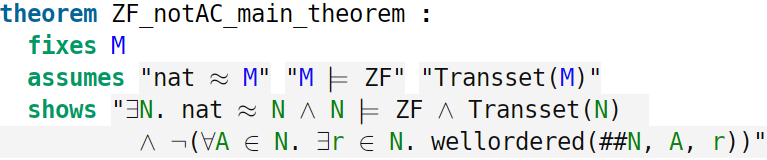
\includegraphics[width=1.1\linewidth]{./images/ZF_notAC_main_theorem.png} 
    \end{figure}

    \vspace{-5pt}
    意味 \\
    {\small
    \hspace{1cm} $M$をZFのc.t.m.とする。このとき、あるZFのc.t.m. $N$\\
    \hspace{1cm} があって、$N$は整列可能定理を満たさない
    }
\end{frame}

\begin{frame}{作業工程}
    以下の工程に分けられる
    {\small
    \begin{itemize}[itemsep=8pt]
        \item symmetric extensionの定義
        \item ZFのモデルであることの証明
        \item 特定のsymmetric extensionの構成
        \item それが$\neg$ACを満たすことの証明
    \end{itemize} }
\end{frame}

\begin{frame}{作業量}
    約1万5千行のコード \hspace{0.6cm} {\small 補題など(3K行)}
    {\small
    \begin{itemize}[itemsep=8pt]
        \item symmetric extensionの定義(3K行)
        \item ZFのモデルであることの証明(5K行)
        \item 特定のsymmetric extensionの構成(2K行)
        \item それが$\neg$ACを満たすことの証明(2K行)
    \end{itemize} 

    ※Isabelle/ZFでの集合論の形式化の各先行研究と同じくらい
    }
\end{frame}

\begin{frame}{困難だった点(1)\, {\normalsize 自明なことの確認が大変}}
    \begin{itemize}[left=0cm]
        \item クラスに「それを表す論理式が存在すること」
        \item 定義した関数が「本当に関数であること」
        \vspace{5pt}
        {\small
        \begin{itemize}
            \item 特に「帰納的に定義された$M$内の関数」の場合
            \vspace{5pt}
            {\begin{itemize}[itemsep=5pt]
                \item 仮定とZFからちゃんと構成できるか?
                \item このような関数を定義するための補題が\\
                      2千行以上
            \end{itemize}}
        \end{itemize}
        }
    \end{itemize}
\end{frame}

\begin{comment}

\begin{frame}{困難だった点(2)\, {\normalsize 先行研究の強制関係の定義}}
    \begin{itemize}[itemsep=9pt]
        \item よくあるfor allに対する強制関係の定義
              $$ p \Vdash \forall x \phi(x, \dot{x_1}, ..., \dot{x_n}) \Leftrightarrow \forall \dot{x} \in M^\Pbb(p \Vdash \phi(\dot{x}, \dot{x_1}, ..., \dot{x_n})) $$
        \item 先行研究{\small [Gunther et al. 20]}の定義
              $$ p \Vdash \forall x \phi(x, \dot{x_1}, ..., \dot{x_n}) \Leftrightarrow \forall x \in \textcolor{red}{M}(p \Vdash \phi(x, \dot{x_1}, ..., \dot{x_n})) $$
              {\small 
                \hspace{0.5cm}※この定義でうまくいくように修正されている
              }
        \item [\textcolor{red}{$\blacktriangleright$}] 強制関係の帰納法に$M \setminus \Pbb$-name以外が混入する...
    \end{itemize}
\end{frame}
\begin{frame}{解決策(2)}
    \begin{itembox}[l]{先行研究{\small [Gunther et al. 20]}の$x_G$の定義}
    {\small
        $x \in M$に対し
        \vspace{-5pt}
        $$x_G := \{ y_G \, | \, y \in \bm{\mathbf{dom}}(x), \exists p \in G. (y, p) \in x \}$$
    }
    \end{itembox}
    \vspace{-1cm}
    {\small 
    \begin{itemize}[itemsep=4pt]    
        \item $x_G$が$M$上の関数になっている
        \item $x \in M$に対し、ある$\dot{z} \in M^\Pbb$があって$x_G = \dot{z}_G$
            \vspace{3pt}
              {\small
              \begin{itemize}
                  \item この事実を形式化し帰納法中で$x$の代わりに$\dot{z}$を使う
                  \item 最終的には解決策(3)で問題の帰納法自体不要に
              \end{itemize}}
    \end{itemize}
    }
\end{frame}

\end{comment}


\begin{frame}{困難だった点(2)\, {\normalsize ZFのモデルであることの証明}}
    \begin{itembox}[l]{命題}
        {\small
            $N$が推移的かつalmost universalなクラスで、$\Delta_0$-separationを\\
            満たすならば、$N$はZFの内部モデルである
        }
    \end{itembox}
    \vspace{-1.2cm}
    {\small
    \begin{itemize}[itemsep=2pt]
        \item 参考文献{\small [Karagila 23]}では、symmetric extensionが\\
              ZFのモデルであることの証明にこの命題を使用
        \item Isabelle/ZF上で、$N$が$M[G]$において「クラスであること」が証明できなかった      
        \begin{itemize}
          \item 論理式を具体的に構成するのが大変すぎる?
        \end{itemize}  
    \end{itemize}
    }
\end{frame}

\begin{frame}{解決策(2)}
    \vspace{-10pt}
    {\small
        \begin{itemize}[itemsep=8pt]
            \item $\bm{\mathbf{HS}}_{\Fcal}$に相対化した強制関係$\textcolor{red}{\Vdash_{\bm{\mathbf{HS}}_{\Fcal}}}$を形式化
                  \begin{itemize}
                      \item 参考資料[Karagila 23]に書かれている概念
                      \item 強制関係の定義の量化の動く範囲を$\bm{\mathbf{HS}}_{\Fcal}$に制限
                      \item $\Vdash_{\bm{\mathbf{HS}}_{\Fcal}}$は、symmetric extensionに対し、\\
                            generic extensionに対する$\Vdash$のように振舞う
                  \end{itemize}
            \item $\Vdash_{\bm{\mathbf{HS}}_{\Fcal}}$を用いてZFのモデルであることを証明
                 % \begin{itemize}
                 %     \item 強制関係の帰納法が不要になり{\footnotesize「困難だった点(2)」}も解決
                 % \end{itemize}
        \end{itemize}
    }
\end{frame}


\section {考察}

\begin{frame}{考察(1) {\normalsize c.t.m.アプローチについて}}
    \vspace{-30pt}
    \,{\small 
    \begin{itemize}
        \item 本研究で形式化したのは、\\
              「ZFのc.t.m.が存在すればZF+$\neg$ACのモデルが存在する」
              \begin{itemize}
                \item 強制法の形式化[Gunther et al. 20]を使うため仮定
              \end{itemize}
        \item 証明したいことは、Con(ZF)$\rightarrow$Con(ZF+$\neg$AC)だが、\\
              ZFのc.t.m.の存在は、Con(ZF)から証明できない
              \begin{itemize} 
                \item このギャップを埋める部分が形式化できていない
                \begin{itemize}
                    \item 本当は形式化したい
                \end{itemize}
              \end{itemize}
    \end{itemize}
    }
\end{frame}

\begin{frame}{形式化できていない部分}
    \,
    {\small 
        以下の形式化ができれば、ZFのc.t.m.の存在の仮定をなくせる

        \textbullet「任意のZFの有限部分$\Delta$に対し、ZFの有限部分$\Gamma$があって\\
                  \,\,\,\,\,\,\,\,\,$\Gamma$のc.t.m.が存在すれば$\Delta + \neg$ACのモデルが存在する」
                  \vspace{-5pt}
                  \begin{itemize}[left=1.5cm]
                    \item [\textasteriskcentered] 今回の形式化を修正すれば可能(ほぼできている)
                  \end{itemize}
        \textbullet 与えられたZFの有限部分$\Gamma$に対し、$\Gamma$のc.t.m.が存在する
                  \vspace{-5pt}
                  \begin{itemize}[itemsep=5pt,left=1.5cm]
                    \item [\textasteriskcentered] ZFモデルの中でZFのモデルを考える必要がある?
                    
                    \,\,\,\,\,\,\,\,\textendash \,\,(労力的に)形式化が厳しそう...
                  \end{itemize}
    }
\end{frame}

\begin{frame}{考察(2) メタ/対象レベル}
    今回、ZFのモデルの中の性質の証明が大変だった
    {\small 
    \begin{itemize}[itemsep=5pt]
        \item コード化された論理式を扱う必要があった
        \item メタレベルで成り立つことを\\
              もう一度証明しなければいけないのもきつい
    \end{itemize}}

    \textcolor{red}{\blacktriangleright}{\small 
    メタ/対象レベルの証明を同時に書ける or\\
    \,\,\,\,\,\,他方に変換できるような機能があると嬉しい}

    \textcolor{red}{\blacktriangleright}{\small 
    今回のテーマに限らず、数学基礎論の形式化には便利そう} 
\end{frame}

\begin{frame}{まとめ}
    $\neg$ACの相対無矛盾性証明をIsabelle/ZFで形式化
    {\small
    \begin{itemize}[itemsep=8pt]
        \item ZFのc.t.m.から出発し、\\ZF+$\neg$ACをみたすsymmetric extensionを構成
        \item c.t.m.に関する形式化できていない部分がある
        \item 参考資料の通りにいかず試行錯誤した部分も
        \item メタ/対象レベルの形式的証明を「つなげる」機能がほしい
    \end{itemize}
    }
\end{frame}

\appendix
\setbeamertemplate{footline}{}
 
\begin{frame}{参考文献(1)}
    \vspace{-30pt}
    \, {\footnotesize 
    \begin{itemize}[itemsep=5pt, left=0pt]
        \item K. Kunen, Set Theory An Introduction To Independence Proofs, North-Holland, 1980 \\
              日本語訳: 藤田 博司 訳, 集合論: 独立性証明への案内, 日本評論社, 2008
        \item T. Jech, Set Theory: The Third Millennium Edition, Springer, 2002
        \item T. Jech, The Axiom of Choice, Dover Publications, 2008
        \item A. Karagila, Lecture Notes: Forcing \& Symmetric Extensions, 2023
    \end{itemize}
    }

\end{frame}

\begin{frame}{参考文献(2)}
    \vspace{-30pt}
    \, {\footnotesize 
    \begin{itemize}[itemsep=5pt, left=0pt]
        \item G. Klein et al., seL4: Formal Verification of an OS Kernel, 2014
        \item LC. Paulson, The Relative Consistency of the Axiom of Choice Mechanized Using Isabelle/ZF, 2003
        \item E. Gunther et al., Formalization of Forcing in Isabelle/ZF, 2020
        \item E. Gunther et al., The Independence of the Continuum Hypothesis in Isabelle/ZF, 2022
    \end{itemize}
    }

\end{frame}

\begin{comment}
    \item K. Kunen, Set Theory An Introduction To Independence Proofs, North-Holland, 1980\\
              日本語訳: 藤田 博司 訳, 集合論: 独立性証明への案内, 日本評論社, 2008
        \item T. Jech, Set Theory: The Third Millennium Edition, Springer, 2002
        \item T. Jech, The Axiom of Choice, Dover Publications, 2008
        \item A. Karagila, Lecture Notes: Forcing & Symmetric Extensions, 2023
        \item G. Klein et al., seL4: Formal Verification of an OS Kernel, 2014
        \item LC. Paulson, The Relative Consistency of the Axiom of Choice Mechanized Using Isabelle/ZF, 2003
        \item E. Gunther et al., Formalization of Forcing in Isabelle/ZF, 2020
        \item E. Gunther et al., The Independence of the Continuum Hypothesis in Isabelle/ZF, 2022
\end{comment}

\end{document}


